\documentclass{beamer}
\usepackage[english]{babel}
\usepackage[backend=biber]{biblatex}
\usepackage{bytefield}
\usepackage{csquotes}
\usepackage{gnuplottex}
\usepackage{tikz}
\setbeamertemplate{bibliography item}[text]
\usetikzlibrary{chains, scopes}

\addbibresource{../../references.bib}

\title{SCTP Send buffer Advertising}
\subtitle{CS4099 Project\\
  Final Evaluation}

\author{Arpan Kapoor, Deepak Sirone J, K Prasad Krishnan\\
  Guided By:\\ Dr.~Vinod Pathari\\
  Mr.~V Anil Kumar, Principal Scientist, CSIR, Bengaluru}

\date{April 25, 2016}

\begin{document}

\begin{frame}
  \titlepage
\end{frame}

\begin{frame}{Outline}
  \tableofcontents
\end{frame}

\section{Introduction}
\begin{frame}{\insertsection}

\begin{itemize}
  \item Stream Control Transmission Protocol (SCTP):
  \begin{itemize}
    \item Supports multiple logical channels called streams
    \item Multi-homing
  \end{itemize}
\end{itemize}

\begin{itemize}
  \item Send buffer Advertising:
  \begin{itemize}
    \item specialized chunks will carry the amount of backlogged data
      present in the sender's buffer.
  \end{itemize}
\end{itemize}

\end{frame}

\section{Problem Statement}
\begin{frame}{\insertsection}
  \begin{itemize}
    \item To propose a scheme to
      \begin{itemize}
        \item advertise send buffer occupancy information in SCTP
        \item implement it in the Linux kernel and
        \item study the performance implications of the same.
      \end{itemize}
  \end{itemize}
\end{frame}

\section{Previous Design}
\begin{frame}[fragile]
\frametitle{\insertsection}
  \begin{itemize}
    \item New chunk type with Chunk Type value between 128 to 190.
    \item Highest order 2 bits determine action to be taken if Chunk Type is
      unknown.
    \item This ensures that unmodified hosts won't send a
      Unrecognized Chunk Type Error chunk upon reception.
  \end{itemize}

  \begin{figure}[h]
    \centering
    \begin{bytefield}{32}
    \bitheader{0-31}\\
    \bitbox{8}{Chunk Type} & \bitbox{8}{Chunk Flags} & \bitbox{16}{Chunk Length}\\
    \bitbox{32}{Send buffer size}
    \end{bytefield}
    \caption{Proposed Chunk for send buffer advertisement}
  \end{figure}
\end{frame}

\section{Current Design}
\begin{frame}[fragile]
\frametitle{\insertsection}
  \begin{itemize}
    \item Every SCTP packet having a DATA chunk contains the
      send buffer occupancy percentage chunk as the first chunk.
    \item Traffic controller classification required each packet to have
      the send buffer occupancy information.
  \end{itemize}

  \begin{figure}[h]
    \centering
    \begin{bytefield}{32}
    \bitheader{0-31}\\
    \bitbox{8}{Chunk Type} & \bitbox{8}{\tiny Percentage send buffer occupancy} &
    \bitbox{16}{Chunk Length}\\
    \end{bytefield}
    \caption{Proposed Chunk for send buffer advertisement}
  \end{figure}
\end{frame}

\begin{frame}
  \frametitle{Test bed Design}
  A dumbbell shaped network topology was created with two routers in the center,
  and multiple hosts connected to one end of each router via a switch. This
  ensures that we have a bottleneck link in all flows between end hosts on
  either side.
  \begin{figure}[h]
    \centering
    \small
    \begin{tikzpicture}[scale=0.75,transform shape,start chain=testbed going right]

      \node [on chain] {\vdots};

      \node [start branch=1 going above, on chain,
      label=below:PC\textsubscript{\(1\)},
      label=right:\texttt{\scriptsize 192.168.150.2}] (pc1)
      {
\includegraphics{imgs/pc.eps}};

      \node [start branch=2 going below, on chain,
      label=below:PC\textsubscript{\(x\)},
      label=right:\texttt{\scriptsize 192.168.150.x}] (pcn)
      {
\includegraphics{imgs/pc.eps}};

      \node [on chain, join=with pc1, join=with pcn,
      label=below:Switch\textsubscript{\(1\)}]
      {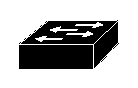
\includegraphics{imgs/switch.eps}};

      \node [on chain, join,
      label=below:RPi\textsubscript{\(1\)}] (rpi1)
      {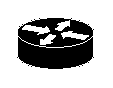
\includegraphics{imgs/router.eps}};

      \node [on chain, join,
      label=below:RPi\textsubscript{\(2\)}] (rpi2)
      {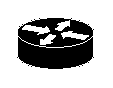
\includegraphics{imgs/router.eps}};

      \draw[-] (4.25, 0) -- (4.25, 0.5)
      node[above] {\scriptsize \texttt{192.168.150.1}};

      \draw[-] (8.45, 0) -- (8.45, 0.5)
      node[above] {\scriptsize \texttt{192.168.50.1}};

      \draw[-] (5.8, 0) -- (5.8, 1.5)
      node[above] {\scriptsize \texttt{192.168.100.2}};

      \draw[-] (6.85, 0) -- (6.85, -1.5)
      node[below] {\scriptsize \texttt{192.168.100.3}};

      \node [on chain, join,
      label=below:Switch\textsubscript{\(2\)}] (switch2)
      {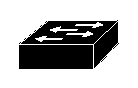
\includegraphics{imgs/switch.eps}};

      \node [on chain] {\vdots};

      \node [start branch=3 going above, on chain, join=with switch2,
      label=below:PC\textsubscript{\(x+1\)},
      label=left:\texttt{\scriptsize 192.168.50.2}]
      {
\includegraphics{imgs/pc.eps}};

      \node [start branch=4 going below, on chain, join=with switch2,
      label=below:PC\textsubscript{\(y\)},
      label=left:\texttt{\scriptsize 192.168.50.y}]
      {
\includegraphics{imgs/pc.eps}};

    \end{tikzpicture}
    \caption{Test bed implementation}
    \label{fig:testbed}
  \end{figure}
\end{frame}

\section{Work Done}
\begin{frame}{\insertsection}
  \begin{itemize}
    \item Modified kernel module \texttt{sctp\_probe} to measure send buffer.
    \item Explored Linux kernel SCTP implementation.
    \item Identified parameter to be advertised.
    \item A patch implementing the SCTP send buffer advertisement was created for
      Linux kernel \texttt{v4.6-rc4}.
    \item The send buffer advertisement chunk type value was set to 150.
    \item A kernel timer was added corresponding to each SCTP association
      (within the \texttt{struct sctp\_association}).
    \item A state table was created for this chunk, specifying the states in which
      the send buffer advertisement chunk should be generated and sent.
  \end{itemize}
\end{frame}

\section{Tests conducted}
\begin{frame}{\insertsection}
  \begin{itemize}
    \item Queueing discipline - Classless \& Classful.
    \item Classless - TBF, SFQ, etc.
    \item Classful - HTB, CBQ, etc.
  \end{itemize}
  AIM - create a classification hierarchy which works better than the existing
  qdiscs.
\end{frame}

\section{Results}
\begin{frame}[fragile,allowframebreaks]{\insertsection}

  \begin{figure}[h]
    \centering
    \begin{gnuplot}[terminal=cairolatex, scale=0.75]
      set xlabel 'Time (s)'
      set ylabel 'Percentage send buffer used'
      set format y '%.0s'
      set key off
      set xrange [0:315]
      plot 'data/deep_tbf.dat' using ($1-5):2 lw 2 with lines,'data/prasad_tbf.dat' using ($1-5):2 lw 2 with lines
    \end{gnuplot}
    \caption{Percentage send buffer variation with 2 flows each having duration of
      300 seconds using the Token Bucket Filter qdisc with rate limited to
      1mbit/sec}
    \label{fig:tbf}
  \end{figure}

  \begin{figure}[h]
    \centering
    \begin{gnuplot}[terminal=cairolatex, scale=0.75]
      set xlabel 'Time (s)'
      set ylabel 'Percentage send buffer used\vspace{0.5cm}'
      set format y '%.0s'
      set key off
      set xrange [0:310]
      plot 'data/deep_sfq.dat' using ($1-80): 2 lw 2 with lines,'data/prasad_sfq.dat' using ($1-80): 2 lw 2 with lines
    \end{gnuplot}
    \caption{Percentage send buffer variation with 2 flows each having duration of
      300 seconds using Stochastic Fair Queuing qdisc with rate limited to
      1mbit/sec}
    \label{fig:sfq}
  \end{figure}

\end{frame}

\section{Work to be completed}
\begin{frame}{\insertsection}
  \begin{itemize}
    \item There are several scheduling algorithms which prioritizes packets based on some
    criteria. One of these priority based scheduling algorithms can be modified to consider
    the send buffer information and to improve QoS for high volume flows.
  \end{itemize}
\end{frame}

\section{References}
\begin{frame}[allowframebreaks]
  \frametitle<presentation>{\insertsection}
  \nocite{*}
  \printbibliography
\end{frame}

\end{document}
